\chapter{数値解析}
\section{利得の比較}
本解析では,ユーザ数$N=2$,セグメント長$T=1$[s],全帯域幅$B = 4$[Mbps] ,ユーザが選択できるビデオビットレート$r_i$は(1,2,3,4,5,6)[Mbps]とした場合を想定した.

図\ref{fig:kisonritoku}と図\ref{fig:teianritoku}は,ユーザ2のビデオビットレートを1Mbpsに固定し,ユーザ1のビデオビットレートを変化させた際の各ユーザの利得遷移を示している.
ユーザ1が高ビットレートを要求するにつれて,帯域幅に影響を与える利己的な要求をするユーザになっていることを表す.一方,ユーザ2は1Mbpsと帯域幅にあまり影響を与えないユーザとした.
図\ref{fig:kisonritoku}では非協力ゲームレート制御法の利得関数\ref{eq:f_{buffer}}から得られる利得の遷移を示す.
図\ref{fig:teianritoku}では提案する利得関数\ref{eq:f_buffi}から得られる利得の遷移を示す.

図\ref{fig:kisonritoku}より非協力ゲームレート制御法\cite{kison}\cite{motomoto}では,ユーザ1のビットレートが増加するにつれ,ユーザ2の利得が大きく減少している.つまり,帯域に影響を与えるユーザ1だけでなく,帯域に影響を与えないユーザ2にも過渡に利得減少を与えている.

一方,提案した利得関数\ref{eq:f_buffi}を用いることで,ユーザ2に対する過渡な制限を回避し,利得の減少を抑制することができた.また,同時に帯域に影響を与えるユーザ1に対して,影響を大きく与える高ビットレートになるにつれて,大きく利得減少を与えている.

これにより,提案する改良法は,各ユーザのビデオビットレートが他ユーザの使用帯域に与える影響を考慮し,特定のユーザへの過渡な利得減少を抑える帯域割り当てを可能にすると言える.

\begin{figure}[tp]
  \centering
  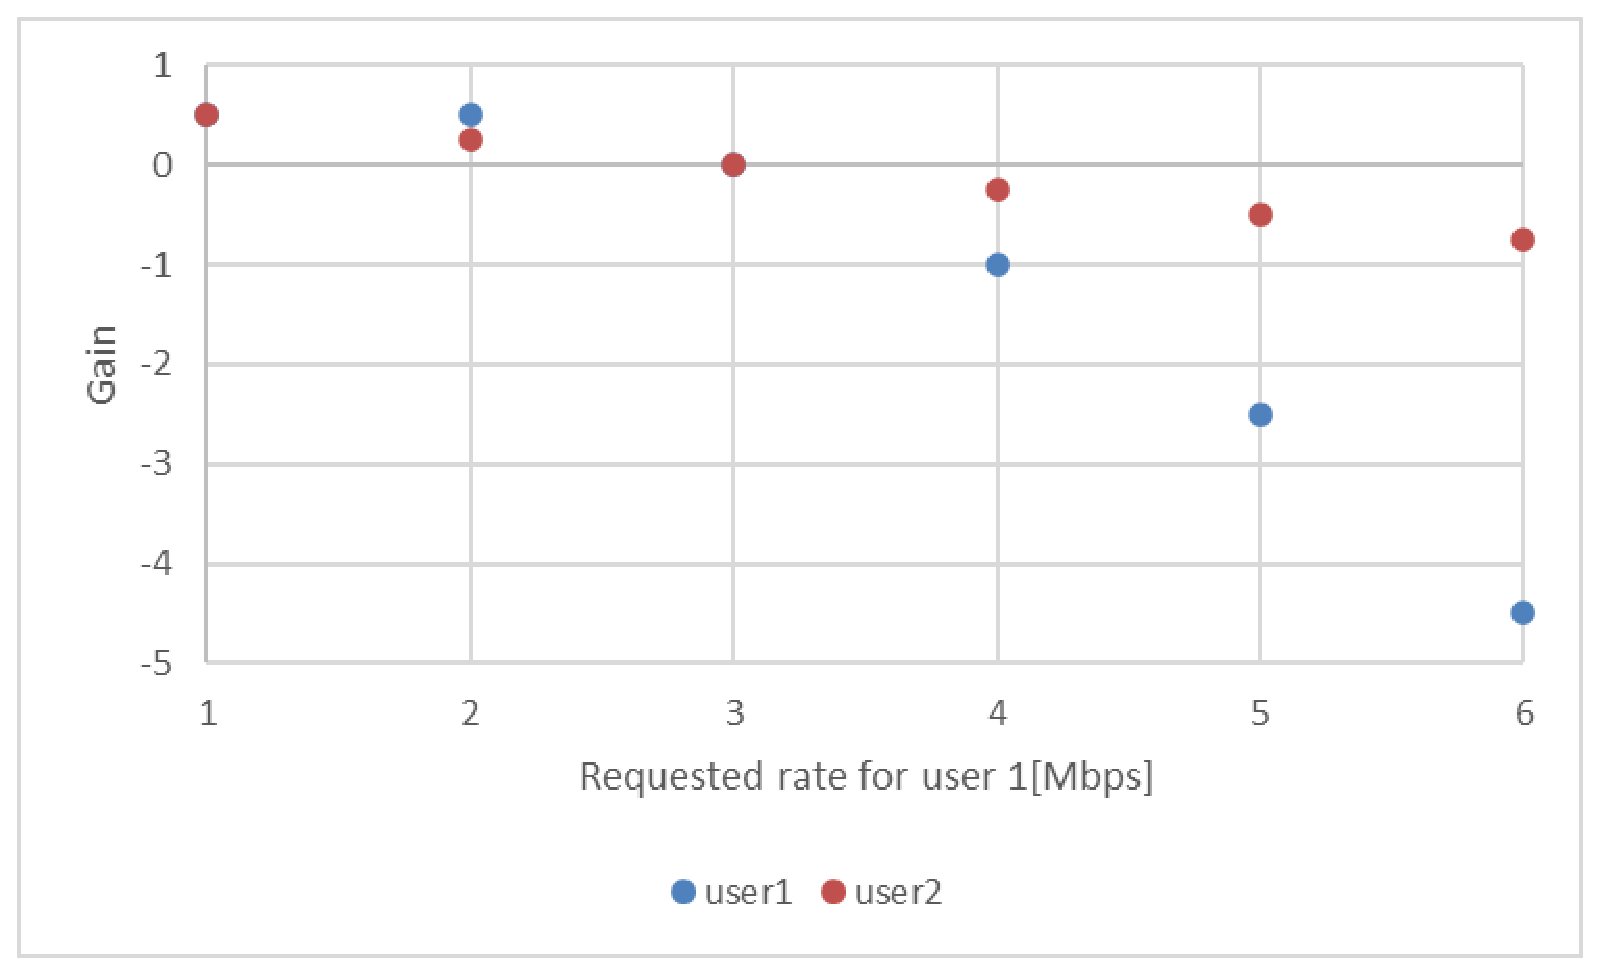
\includegraphics[scale=0.45]{kison.eps}
  \bicaption{ユーザ2が1Mbps要求時の非協力ゲームレート制御法\cite{kison}\cite{motomoto}の利得遷移}%
            {Gain transition of the non-cooperative game rate control method when user 2 requests 1 Mbps}
    \label{fig:kisonritoku}
\end{figure}

\begin{figure}[bp]
  \centering
  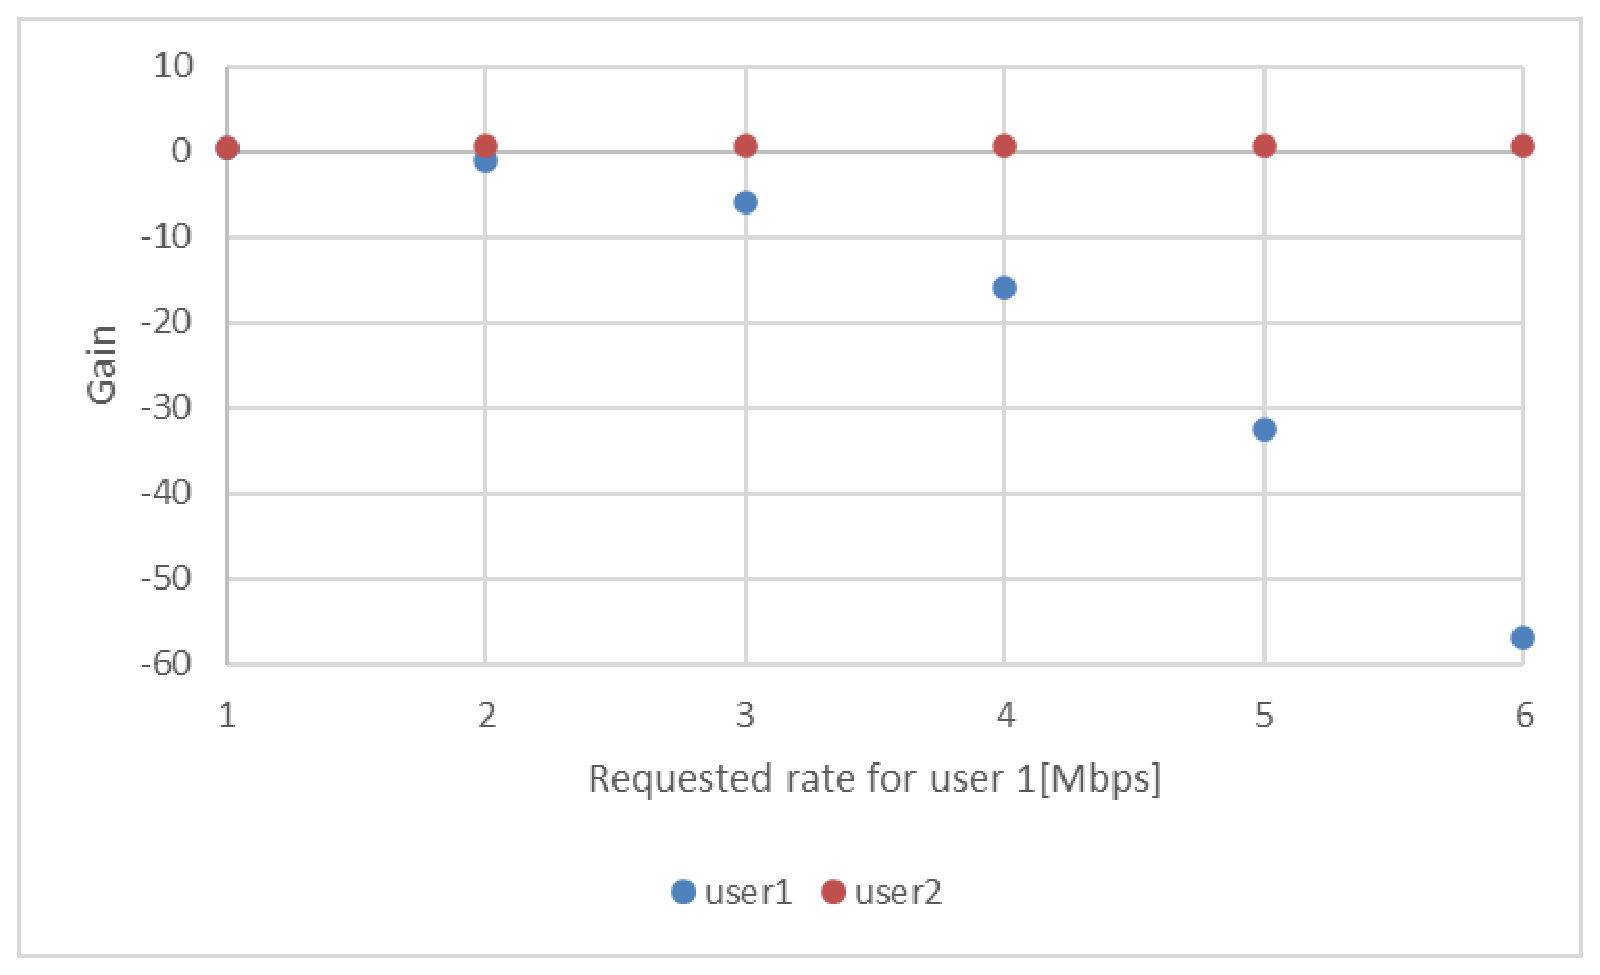
\includegraphics[scale=0.45]{teian.eps}
  \bicaption{ユーザ2が1Mbps要求時の提案関数の利得遷移}%
            {Gain transition of the proposed function when user 2 requests 1 Mbps}
    \label{fig:teianritoku}
\end{figure}


\section{貯蓄バッファ量の比較}

本解析では,4人のユーザが全帯域幅$B = 20$[Mbps]を争ったときの,ユーザの平均貯蓄バッファ量を解析する.
全ユーザが4分間の動画を視聴し,初め4sは動画が再生されず,1Mbpsのビデオビットレートでバッファが貯蓄されることを想定したシミュレーションを行う.
この解析では,式\eqref{eq:syousai}と式\eqref{fig:teianritoku}を用いた以下の式\eqref{eq:proposed}によって最適レートを導出し,その際に貯蓄されるバッファ量の平均を比較する.

\begin{equation}
\begin{split}
  f_i(r_k) = &\ \alpha_{\text{ct}} \log(1 + |\beta_{\text{ct}}| r_{i,k}) \\
  &+ \mu \left( \frac{2 e^{p(b_{i,k-1} - b_s)}}{1 + e^{p(b_{i,k-1} - b_s)}} T r_{i,k} \right) - \mu \omega T \left(\frac{r_{i,k}^2}{B\left(1-\frac{r_{i,k}}{\sum^N_{j=1}r_{j,k}}\right)}\right) \\
  &+ \gamma_i \left( -m(r_{i,k} - r_{i,k-1} + r^{(J)})^2 - 2m(r_{i,k} - r_{i,k-1}) \right)
  \label{eq:proposed}
\end{split}
\end{equation}

以下に,表\ref{tab:parameters}に各パラメータの値と,表\ref{tab:bitrates}にユーザが要求できるレートを示す.

\begin{table}[h!]
\centering
\bicaption{各パラメータの値\cite{kison}}
            {Value of parameter\cite{kison}}
\label{tab:parameters}
\begin{tabular}{cc}
\toprule
\textbf{Parameter} & \textbf{Value} \\
\midrule
$\alpha$ & 0.5124 \\
$\beta$ & -2.7524 \\
$N$ & 4 \\
$T$ & 2 s \\
$B_W$ & 20 Mbps \\
$J$ & 21 \\
$\mu$ & $3.2 \times 10^{-6}$ \\
$\omega$ & 1.25 \\
$\gamma_i$ & $1.0 \times 10^{20}$ \\
$p$ & 0.05 \\
$m$ & $1.0 \times 10^{-6}$ \\
\bottomrule
\end{tabular}
\end{table}

\begin{table}[h!]
\centering
\bicaption{ユーザが要求可能なビデオビットレート\cite{kison}}
            {User-requestable video bit rate\cite{kison}}
\label{tab:bitrates}
\begin{tabular}{ll}
\toprule
\textbf{Resolution} & \textbf{Bit rate (Mbps)} \\
\midrule
$480 \times 360$ & 0.1, 0.2, 0.3, 0.4 \\
$704 \times 480$ & 0.5, 0.6, 0.7, 0.9, 1.0 \\
$1280 \times 720$ & 1.2, 1.5, 2.0, 2.5, 3.0, 3.5, 4.0, 4.5, 5.0, 5.5, 6.0 \\
\bottomrule
\end{tabular}
\end{table}

図\ref{fig:hiritu}は,シミュレーション結果の平均貯蓄バッファ量を示している.縦軸が平均貯蓄バッファ量を表し,横軸にユーザを表している.


\begin{figure}[h]
  \centering
  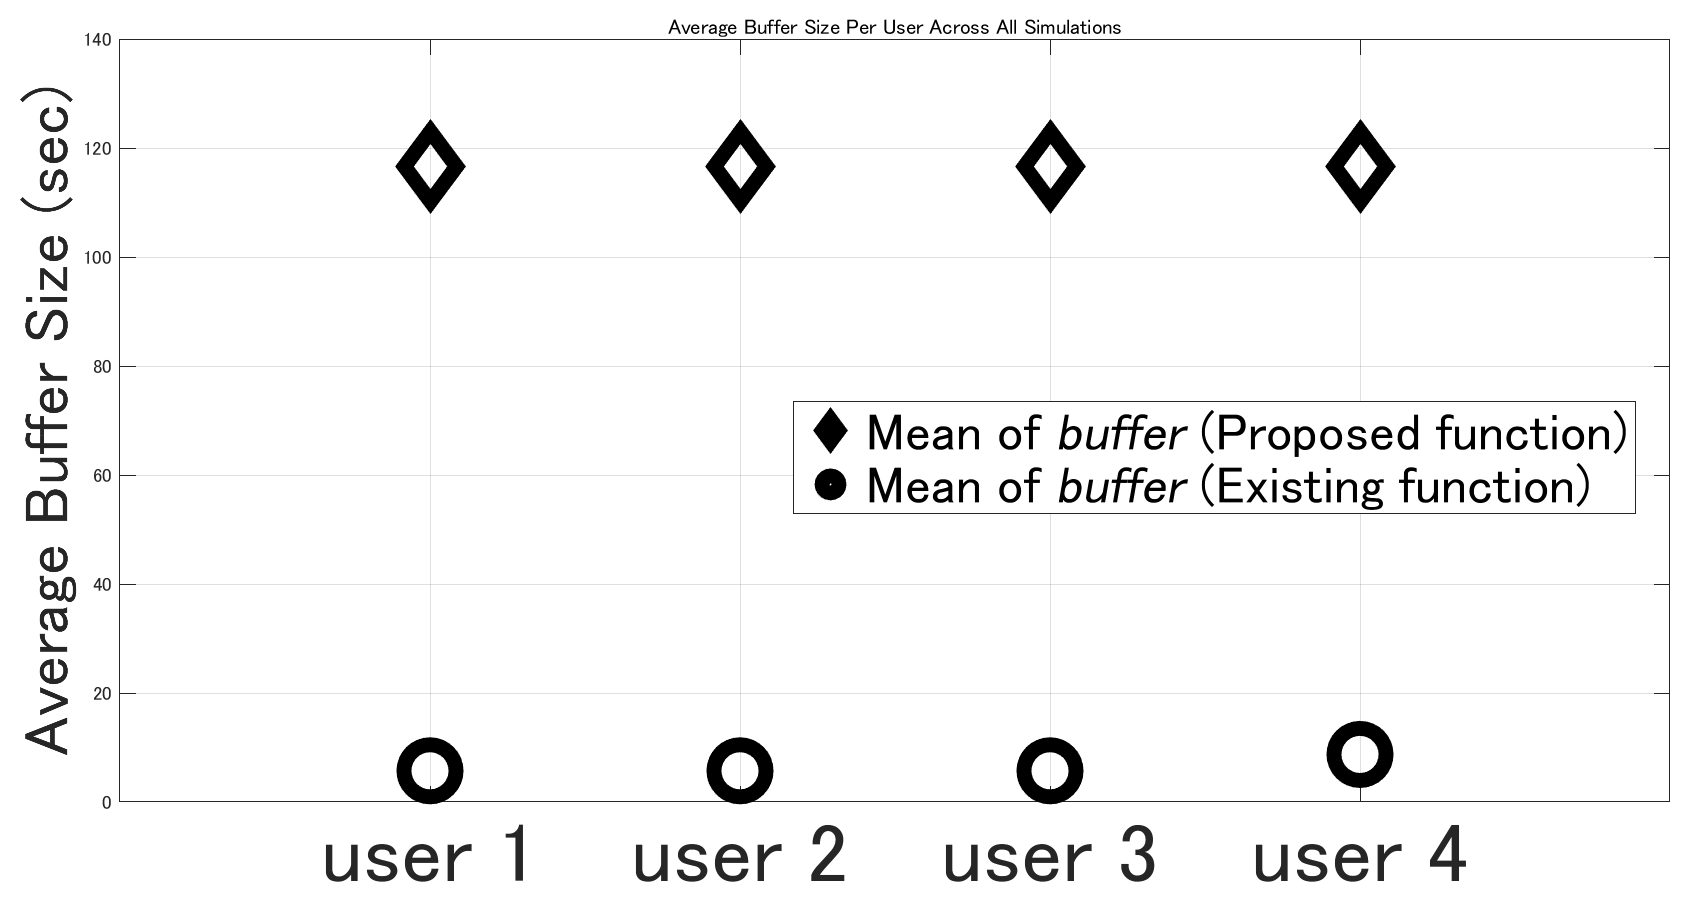
\includegraphics[scale=0.45]{hiritu_buffer.eps}
  \bicaption{平均貯蓄バッファ量の比較}%
            {Comparison of Average Savings Buffers}
    \label{fig:hiritu}
\end{figure}

図\ref{fig:hiritu}よりどのユーザにおいても,非協力ゲームレート制御\cite{kison}の利得関数\ref{eq:syousai}によって貯蓄されるバッファ量より,提案利得関数\ref{eq:proposed}によって貯蓄されるバッファ量の方が多いことが分かる.

これにより,提案する改良法は,非協力ゲームレート制御\cite{kison}よりバッファ枯渇による動画の再生中断が起こりにくいと言える.